%\documentclass{article}
\documentclass[10pt,a4paper]{report}
\usepackage[a4paper,bindingoffset=0.2in,%
            left=1in,right=1in,top=1in,bottom=1in,%
            footskip=.25in]{geometry}

\usepackage[utf8]{inputenc}

\title{Solutions}
\author{C Thierfelder}
\date{June 2024}


%MATH
\usepackage{amsmath}
\usepackage{amsfonts}
\usepackage{amsthm}
\usepackage{units}
\usepackage{mathrsfs}

\usepackage{hyperref}


\newtheorem{remark}{Remark}[section]
\theoremstyle{definition}
\newtheorem{definition}{Definition}[section]
\newtheorem{theorem}{Theorem}[section]

\DeclareMathOperator{\Aut}{Aut}
\DeclareMathOperator{\GL}{GL}

%PAGELAYOUT
\usepackage{a4wide}

%GRAPHICS
\usepackage{graphicx}
\usepackage[dvipsnames]{xcolor}
\usepackage{tikz}
\usepackage[outline]{contour} % glow around text

\usetikzlibrary{shapes}
\usetikzlibrary{plotmarks}
\usetikzlibrary{decorations.markings}

\usepackage{pgfplots}
\usepgfplotslibrary{polar}

%HYPERLINKS
\usepackage{hyperref}
\hypersetup{
    colorlinks=true,
    linkcolor=blue,
    filecolor=magenta,      
    urlcolor=cyan,
}

\usepackage[shortlabels]{enumitem}

\usepackage{etoolbox}
\providetoggle{includeCoverPic}
\settoggle{includeCoverPic}{true}
%\settoggle{includeCoverPic}{false}
\usepackage{subfiles}

\tikzset{>=latex} % for LaTeX arrow head
\colorlet{myred}{red!85!black}
\colorlet{mydarkred}{red!55!black}
\colorlet{mylightred}{red!85!black!12}
\colorlet{myfieldred}{mydarkred!5} % for S' background
\colorlet{myredhighlight}{myred!20} % highlights simultaneity in ladder paradox
\colorlet{myblue}{blue!80!black}
\colorlet{mydarkblue}{blue!50!black}
\colorlet{mylightblue}{blue!50!black!30}
\colorlet{mylightblue2}{myblue!10}
\colorlet{mygreen}{green!80!black}
\colorlet{mypurple}{blue!40!red!80!black}
\colorlet{mydarkgreen}{green!50!black}
\colorlet{mydarkpurple}{blue!40!red!50!black}
\colorlet{myorange}{orange!40!yellow!95!black}
\colorlet{mydarkorange}{orange!40!yellow!85!black}
\colorlet{mybrown}{brown!20!orange!90!black}
\colorlet{mydarkbrown}{brown!20!orange!55!black}
\colorlet{mypurplehighlight}{mydarkpurple!20} % highlights simultaneity in ladder paradox
\tikzstyle{world line}=[myblue!40,line width=0.3]
\tikzstyle{world line t}=[mypurple!50!myblue!40,line width=0.3]
\tikzstyle{world line'}=[mydarkred!40,line width=0.3]
\tikzstyle{mysmallarr}=[-{Latex[length=3,width=2]},thin]
\tikzstyle{mydashed}=[dash pattern=on 3 off 3]
\def\Nsamples{100}
\tikzstyle{vector}=[->,line width=1,line cap=round]
\tikzstyle{vector'}=[vector,shorten >=1.2]
\tikzstyle{particle}=[mygreen,line width=0.9]

\begin{document}

\maketitle

\chapter{Relativistic Quantum Field Theory 1B WS2022/23}
\section{Sheet 1 — Exercise 1 (Lagrangian and Hamiltonian formalism, constrained systems)}
Good exposition: {\sc Hanson, Regge, Teitelboim} - Constrained Hamiltonian Systems - Accademia Nazionale dei Lincei (1976)
\begin{enumerate}[a)]
\item Free non-interacting particles

Euler-Lagrange Eqn:
\begin{align}
\ddot{q}_1=0,\qquad \ddot{q}_1=0
\end{align}
Solutions $q_1(0),q_2(0),\dot{q}_1(0),\dot{q}_2(0)\in\mathbb{R}$:
\begin{align}
q_1(t)=v_1t+s_1,\qquad q_2(t)=v_2t+s_2
\end{align}
Momenta:
\begin{align}
p_1=\frac{\partial L}{\partial q_1}=m_1\dot{q}_1,\qquad p_2=m_1\dot{q}_1\\
\rightarrow \dot{q}_1=\frac{p_1}{m_1},\qquad \dot{q}_1=\frac{p_1}{m_1}
\end{align}
Also $\frac{dp_1}{dt}=0=\frac{dp_2}{dt}$ so $p_1, p_2$ are conserved quantities.

Hamiltonian
\begin{align}
H&=p_1\dot{q}_1+p_2\dot{q}_2-L\\
&=\frac{p_1^2}{2m_1}+\frac{p_2^2}{2m_2}
\end{align}
Necessary and sufficient condition for a constraint is $\det M = 0$ which is not the case
\begin{align}
M_{ij}&=\frac{\partial p_i}{\partial \dot{q}_j}=\left(\begin{array}{cc}
m_1 & 0\\
0 & m_2
\end{array}\right)\\
\text{det}M&=m_1m_2
\end{align}

\item Free particle $q_1'=q_1-q_0$
\begin{align}
L&=\frac{m_1}{2}(\dot{q}_1-\dot{q}_0)^2\\
&=\frac{m_1}{2}\dot{q}_1^2+\frac{m_1}{2}\dot{q}_0^2-m\dot{q}_1\dot{q}_0
\end{align}
Invarianz trafo (gives free particle + total time derivative)
\begin{align}
&=L'+\frac{d\Lambda(q_0,q_1,t)}{dt}\\
&=L'+\frac{\partial\Lambda}{\partial q_1}\frac{\partial q_1}{\partial t}+\frac{\partial\Lambda}{\partial t}\\
&\rightarrow \frac{\partial\Lambda}{\partial q_1}=-m\dot{q}_0,\qquad \frac{\partial\Lambda}{\partial t}=\frac{1}{2}m\dot{q}_0^2
\end{align}
which implies
\begin{align}
\ddot{q}_0&=0\\
\rightarrow q_0&=\alpha+\beta t\\
\rightarrow \Lambda&=-m\beta q_1+\frac{1}{2}m\beta^2t
\end{align}


Euler-Lagrange equations
\begin{align}
\ddot{q}_1-\ddot{q_0}=0,\qquad\ddot{q}_0-\ddot{q_1}=0\\
\rightarrow \frac{\partial^2}{\partial t^2}(q_1-q_0)=0
\end{align}
Solution
\begin{align}
q_1(t)-q_0(t)=vt+s
\end{align}
Momenta
\begin{align}
p_1&=m_1(\dot{q}_1-\dot{q}_0),\qquad p_0=m_1(\dot{q}_0-\dot{q}_1)=-p_1\qquad\text{(constraint)}\\
&\rightarrow p_1-p_0=2m_1(\dot{q}_1-\dot{q}_0)\\
&\rightarrow p_1=m_1(\dot{q}_1-\dot{q}_0)\\
\end{align}
Also $\frac{dp_1}{dt}=0=\frac{dp_0}{dt}$ so $p_1, p_0$ are conserved quantities.


Hamiltonian (canonical momenta are not independent)
\begin{align}
H&=p_1\dot{q}_1+p_0\dot{q}_0-L\\
&=p_1(\dot{q}_1-\dot{q}_0)-L\\
&=\frac{p_1^2}{m_1}-\frac{m_1}{2}\frac{p_1^2}{m_1^2}\\
&=\frac{p_1^2}{2m}
\end{align}
\begin{align}
M_{ij}&=\frac{\partial p_i}{\partial \dot{q}_j}=\left(\begin{array}{cc}
m_1 & -m_1\\
-m_1 & m_1
\end{array}\right)\\
\text{det}M&=0
\end{align}

\item Euler-Lagrange equation
\begin{align}
m_1\ddot{q}_1+\dot{q}_B=0,\qquad \dot{q}_1-\frac{q_B}{m_2}=0\\
\rightarrow (m_1+m_2)\ddot{q}_1=0,\qquad q_B=m_2\dot{q}_1
\end{align}
Solution
\begin{align}
q_1(t)&=\alpha t+\beta\\
q_B(t)&=\alpha m_2
\end{align}
Momenta
\begin{align}
p_1&=m_1\dot{q}_1+q_B\\
p_B&=0\qquad\text{(constraint)}
\end{align}
Also $\frac{dp_1}{dt}=0$ so $p_1$ is a conserved quantity.


Hamiltonian (only one canonical momentum)
\begin{align}
H&=p_1\dot{q}_1+p_B\dot{q}_B-L\\
&=p_1\frac{p_1-q_B}{m_1}-\frac{m_1}{2}\left(\frac{p_1-q_B}{m_1}\right)^2+\frac{1}{2m_2}q_B^2-q_B\frac{p_1-q_B}{m_1}\\
&=\frac{p_1^2}{2m_1}-\frac{p_1q_B}{m_1}+\frac{m_1+m_2}{2m_1m_2}q_B^2\\
&=\frac{p_1^2}{2m_1}+\left(\frac{m_1+m_2}{2m_2}q_B-p_1\right)\frac{q_B}{m_1}\\
\end{align}
\begin{align}
M_{ij}&=\frac{\partial p_i}{\partial \dot{q}_j}=\left(\begin{array}{cc}
m_1 & 0\\
0 & 0
\end{array}\right)\\
\text{det}M&=0
\end{align}

\end{enumerate}

\section{Sheet 1 — Exercise 2 (Theory of relativity, notation)}
\begin{enumerate}[a)]
\item 4-vectors transforming under LT as
\begin{align}
y'=\Lambda y
\end{align}
More mathematical: 4-vector is an element of a four-dimensional vector space considered as a representation space of the standard ($1/2,1/2$) of the Lorentz group. 
\begin{align}
x^\mu&\equiv(t,\mathbf{x})\qquad\text{with}\quad \eta_{\alpha\beta}dx^\alpha dx^\beta=dx^\beta dx_\beta=ds^2=dx'^\mu dx'_\mu=\eta_{\mu\nu}\Lambda^\mu_{\;\alpha}dx^\alpha \Lambda^\nu_{\;\beta}dx^\beta\\
&\rightarrow\quad\eta_{\alpha\beta}=\eta_{\mu\nu}\Lambda^\mu_{\;\alpha} \Lambda^\nu_{\;\beta}\\
u^\mu&=\frac{dx^\mu}{d\tau}=\frac{dx^\mu}{dt}\frac{dt}{d\tau}=(1,\mathbf{v})\gamma\qquad\text{with}\qquad u^\mu u_\mu=1\\
p^\mu&=mu^\mu=(\sqrt{m^2+\mathbf{p}^2},\vec{p})\qquad\text{with}\qquad p^\mu p_\mu=m^2\\
\partial_\mu&=\frac{\partial}{\partial x^\mu}\\
A^\mu&=(\Phi,\mathbf{A})\\
F^{\mu\nu}&=\eta^{\mu\alpha}\eta^{\nu\beta}(\partial_\alpha A\beta-\partial_\beta A\alpha)\\
j^\mu&=(\rho,\mathbf{j})
\end{align}

\item Good summary of all effects: {\sc Sexl, Urbantke} - Relativitaet, Gruppen, Teilchen. Obviously all effects can be explained by a proper Minkowski diagram (important: unit scaling in the different inertial systems are given green and blue hyperbola) \\
\begin{center}
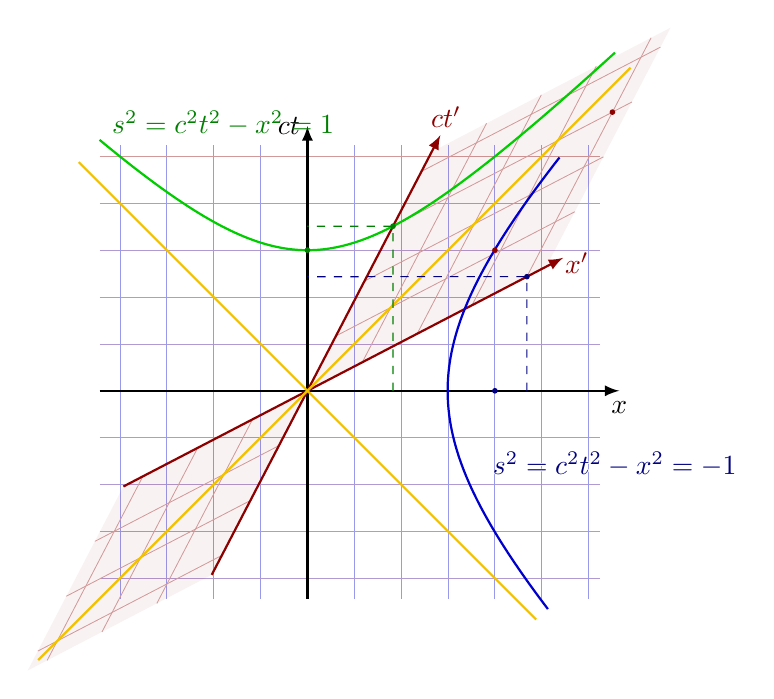
\begin{tikzpicture}[scale=1.2][!]
  \message{Invariant hyperboloids^^J}
  
  % SETTINGS
  \def\xmin{2.2}
  \def\xmax{3.1}
  \def\ymin{2.2}
  \def\ymax{2.6}
  \def\xmaxp{2.85} % maximum of rotated axis
  \def\Nlines{4} % number of world lines (at constant x/t)
  \pgfmathsetmacro\ang{atan(0.52)} % angle between x and x' axes
  \pgfmathsetmacro\d{0.64*\xmax/\Nlines} % grid size
  \pgfmathsetmacro\D{\d/cos(\ang)/sqrt(1-tan(\ang)^2)} % grid size, boosted
  \pgfmathsetmacro\dextra{(\Nlines+1)*\d} % extra line
  \pgfmathsetmacro\st{3*\d} % spacetime interval
  \pgfmathsetmacro\sx{4*\d} % spacetime interval
  \pgfmathsetmacro\sr{sqrt(\sx^2-\st^2)} % spacetime interval sr^2 = st^2 - sx^2 < 0
  \pgfmathsetmacro\Ax{3*\D*sin(\ang)} % x coordinate of event A
  \pgfmathsetmacro\Ay{3*\D*cos(\ang)} % y coordinate of event A
  \pgfmathsetmacro\Bx{4*\D*cos(\ang)} % x coordinate of event B
  \pgfmathsetmacro\By{4*\D*sin(\ang)} % y coordinate of event B
  \pgfmathsetmacro\Cx{\Ay+\By} % x coordinate of event C' %(\Bx+tan(\ang)*\Ay)/sqrt(1-tan(\ang)^2)
  \coordinate (O)  at (0,0);
  \coordinate (X)  at (\xmax+0.2,0);
  \coordinate (T)  at (0,\ymax+0.2);
  \coordinate (X') at (\ang:\xmaxp+0.2);
  \coordinate (T') at (90-\ang:\xmaxp+0.2);
  \coordinate (A)  at (0,\st);        % event A
  \coordinate (A') at (90-\ang:3*\D); % event A', boosted A
  \coordinate (B)  at (\sx,0);        % event A
  \coordinate (B') at (\ang:4*\D);    % event A', boosted A
  \coordinate (C)  at (4*\d,3*\d);    % event C
  
  % WORLD LINE GRID
  \message{  Making world lines...^^J}
  \foreach \i [evaluate={\x=\i*\d;}] in {1,...,\Nlines}{
    \message{  Running i/N=\i/\Nlines, x=\x...^^J}
    \draw[world line]   (-\x,-\ymin) -- (-\x,\ymax);
    \draw[world line]   ( \x,-\ymin) -- ( \x,\ymax);
    \draw[world line t] (-\xmin,-\x) -- (\xmax,-\x);
    \draw[world line t] (-\xmin, \x) -- (\xmax, \x);
  }
  \draw[world line]    (\dextra,-\ymin)  -- (\dextra,\ymax);
  \draw[world line]    (\dextra+\d,-\ymin) -- (\dextra+\d,\ymax);
  %\draw[world line'] (-\xmin,-\dextra) -- (\xmax,-\dextra);
  \draw[world line'] (-\xmin,\dextra) -- (\xmax,\dextra);
  
  % BOOSTED WORLD LINE GRID
  \message{  Making world lines for boosted frame...^^J}
  \fill[mydarkred,opacity=0.05]
    (O) --++ (\ang:\xmaxp) --++ (90-\ang:\xmaxp) --++ (\ang:-\xmaxp) -- cycle;
  \fill[mydarkred,opacity=0.05]
    (O) --++ (\ang:\D-\xmaxp) --++ (90-\ang:\D-\xmaxp) --++ (\ang:\xmaxp-\D) -- cycle;
  \foreach \i [evaluate={\x=\i*\D;}] in {1,...,\Nlines}{
    \message{  Running i/N=\i/\Nlines, x=\x...^^J};
    \ifnumcomp{\i}{<}{\Nlines}{
      \draw[world line'] (\ang:-\x) --++ (90-\ang:\D-\xmaxp);
      \draw[world line'] (90-\ang:-\x) --++ (\ang:\D-\xmaxp);
    }{}
    \draw[world line'] (\ang:\x) --++ (90-\ang:\xmaxp);
    \draw[world line'] (90-\ang:\x) --++ (\ang:\xmaxp);
  }
  
  % AXES
  \draw[->,thick] (0,-\ymin) -- (T) node[left=-1] {$ct$};
  \draw[->,thick] (-\xmin,0) -- (X) node[below=0] {$x$};
  \draw[->,thick,mydarkred] (90-\ang:\D-\xmaxp) -- (T')
    node[right=2,above=-1] {$ct'$};
  \draw[->,thick,mydarkred] (\ang:\D-\xmaxp) -- (X') node[below=2,right=-3] {$x'$};
  
  % LIGHTCONE
  \draw[myorange,thick]
    (-1.1*\xmin,1.1*\xmin) -- (1.1*\ymin,-1.1*\ymin)
    (-\xmaxp,-\xmaxp) -- (1.2*\xmaxp,1.2*\xmaxp);
  
  % SPACELIKE HYPERBOLOIDS
  \draw[mygreen,thick,samples=\Nsamples,smooth,variable=\x,domain=-\xmin:1.05*\xmax]
    plot(\x,{sqrt((\st)^2+(\x)^2)});
%  \draw[mydarkgreen,very thick,samples=\Nsamples,variable=\x,domain=0:\Ax,
%        decoration={markings,mark=at position 0.58 with %{\arrow{latex}}},postaction={decorate}]
%    plot(\x,{sqrt((\st)^2+(\x)^2)});
  \node[mydarkgreen,right=1,above right=0] at (-\xmin,\ymax)
    {$s^2 = c^2t^2-x^2=1$};
  
  % TIMELIKE HYPERBOLOIDS
%  \draw[myred,very thick,samples=\Nsamples,variable=\y,domain=\st:\Cx,
%        decoration={markings,mark=at position 0.58 with %{\arrow{latex}}},postaction={decorate}]
%    plot({sqrt(\sr^2+(\y)^2)},\y);
  \draw[myblue,thick,samples=\Nsamples,smooth,variable=\y,domain=-1.05*\ymin:0.95*\ymax]
    plot({sqrt(\sx^2+(\y)^2)-0.5},\y);
%  \draw[mydarkblue,very thick,samples=\Nsamples,variable=\y,domain=0:\By,
%        decoration={markings,mark=at position 0.58 with %{\arrow{latex}}},postaction={decorate}]
%    plot({sqrt(\sx^2+(\y)^2)-0.5},\y);
  \node[mydarkblue,right=0] at (0.6*\xmax,-0.25*\xmax)
    {\contour{white}{$s^2 = c^2t^2-x^2=-1$}};
  
  % TICKS
  \draw[mydarkgreen,dashed] ({\Ax},0) -- (A') -- (0,{\Ay});
  \draw[mydarkblue,dashed] ({\Bx},0) -- (B') -- (0,{\By});
%  \tick{0,\st}{0} node[mydarkgreen,right=4,below left=-2.5] {$ct_1$};
%  \tick{\sx,0}{90} node[mydarkblue,below=1,below left=-3] {$x_1$};
%  \tick{0,\Ay}{0} node[mydarkgreen,above=1,left=-2]
%    {\contour{white}{$ct_1\cosh\phi$}};
%  \tick{\Ax,0}{90} node[mydarkgreen,right=4,below=-4]
%    {\contour{white}{$ct_1\sinh\phi$}};
%  \tick{\Bx,0}{90} node[mydarkblue,right=9,below=-4]
%    {\contour{white}{$x_1\cosh\phi$}};
%  \tick{0,\By}{0} node[mydarkblue,below=1,left=-2]
%    {\contour{white}{$x_1\sinh\phi$}};
  
  % EVENTS
  \fill[mydarkgreen] (A)  circle(0.03); % event A
  \fill[mydarkgreen] (A') circle(0.03); % event A'
  \fill[mydarkblue]  (B)  circle(0.03); % event B
  \fill[mydarkblue]  (B') circle(0.03); % event B'
  \fill[mydarkred]   (C)  circle(0.03); % event C
  \fill[mydarkred] (\ang:4*\D)++(90-\ang:3*\D) coordinate (C') circle(0.03); % event C'
  %\node[mydarkred,above=2,right=6] at (C') {$\left\{\begin{aligned}
  %  ct' &= ct\cosh\phi -  x\sinh\phi \\
  %   x' &=  x\cosh\phi - ct\sinh\phi
  %\end{aligned}\right.$};
  
\end{tikzpicture}
\end{center}


\end{enumerate}


\section{Sheet 1 — Exercise 3 (Localization of relativistic particles)}
\begin{enumerate}[a)]
\item Pair production - locate particle smaller then the Compton wavelenth $\lambda_C=\hbar/mc$. Back of the envelope estimate
\begin{align}
E=\sqrt{m^2c^2+p^2c^2}\qquad&\rightarrow\Delta p\geq mc\\
\Delta x \cdot\Delta p\geq\frac{\hbar}{2}\qquad&\rightarrow\Delta x \simeq\frac{\hbar}{2mc}
\end{align}
\begin{itemize}
\item Top quark $7\cdot10^{-18}$m
\item Proton $1.3\cdot10^{-13}$m
\item Electron $2.4\cdot10^{-12}$m
\item Hydrogen $1.3\cdot10^{-13}$m
\end{itemize}

\item
\begin{itemize}
\item Top quark $\Delta x $ {\bf kind of similar} to physical size ($10^{-19}$m)
\item Proton $\Delta x $ {\bf larger} than physical size ($0.8\cdot10^{-15}$m)
\item Electron $\Delta x $ {\bf larger} than physical size of 0m (point)
\end{itemize}

\item \textcolor{red}{NOT DONE YET}

\end{enumerate}

\section{Sheet 2 — Exercise 1 (Schroedinger field quantization)}
\begin{enumerate}[a)]
\item Canonical variables $\psi,\psi^*$
\begin{align}
\pi&=i\psi^*\\
\pi^*&=0\qquad \text{(constraint)}
\end{align}
Then
\begin{align}
\mathcal{H}
&=\pi\dot\psi+\pi^*\dot\psi^*-\mathcal{L}\\
&=\frac{1}{2m}(\nabla\psi^*)(\nabla\psi)+V\psi^*\psi\\
&=-\frac{i}{2m}(\nabla\pi)(\nabla\psi)-iV\pi\psi\\
H&=-i\int d^3x \left(\frac{1}{2m}(\nabla_x\pi(x))(\nabla_x\psi(x))+V\pi(x)\psi(x)\right)\\
&=-i\int d^3x \left(-\frac{1}{2m}\pi(x)(\triangle_x\psi(x))+V\pi(x)\psi(x)\right)
\end{align}
Using the standard commutators
\begin{align}
[\psi(x),\pi(y)]=i\delta^{(3)}(x-y),\qquad
[\psi(x),\psi(y)]=0,\qquad
[\pi(x),\pi(y)]=0
\end{align}
Heisenberg equations
\begin{align}
i\partial_t\psi(y)
&=i\int d^3x \frac{1}{2m}\pi(x)(\triangle_x\psi(x))\psi(y)-\frac{1}{2m}\psi(y)\pi(x)(\triangle_x\psi(x))-V(x)\pi(x)\psi(x)\psi(y)+V(x)\psi(y)\pi(x)\psi(x)\\
&=i\int d^3x \frac{1}{2m}\pi(x)(\triangle_x\psi(x))\psi(y)-\frac{1}{2m}(\pi(x)\psi(y)-i\delta^{(3)}(x-y))(\triangle_x\psi(x))\\
&\qquad\qquad\qquad-V(x)\pi(x)\psi(x)\psi(y)+V(x)(\pi(x)\psi(y)-i\delta^{(3)}(x-y))\psi(x)\\
&=i\int d^3x -\frac{1}{2m}(-i\delta^{(3)}(x-y))(\triangle_x\psi(x))-V(-i\delta^{(3)}(x-y))\psi(x)\\
&=-\int d^3x \frac{1}{2m}\delta^{(3)}(x-y)(\triangle_x\psi(x))-V(x)\delta^{(3)}(x-y)\psi(x)\\
&=-\frac{1}{2m}\triangle_y\psi(y)+V(y)\psi(y)
\end{align}
which looks like the one particle Schroedinger equation.
\item
\item
\item
\item
\end{enumerate}

\section{Sheet 11 — Exercise 3 (Integrals in $D$ dimensions)}
\begin{enumerate}[a)]
\item Let's start with 
\begin{align}
\pi^{D/2}
&\equiv\left(\int e^{-k^2}dk\right)^D\\
&=\int e^{-k_1^2}dk_1...\int e^{-k_D^2}dk_D\\
&=\int e^{-k_1^2-..k_D^2}dk_1...dk_D\\
&=\int_0^\infty\int_{\partial S_D} e^{-k^2}k^{D-1}dk d\Omega_D\\
&=\int_0^\infty e^{-k^2}k^{D-1}dk\cdot\int_{\partial S_D} d\Omega_D\\
&=\int_0^\infty e^{-t}t^{(D-1)/2}\frac{dt}{2\sqrt{t}}\cdot\int_{\partial S_D} d\Omega_D\\
&=\frac{1}{2}\int_0^\infty e^{-t}t^{(D/2-1)}dt\cdot\int_{\partial S_D} d\Omega_D\\
&=\frac{1}{2}\Gamma(D/2)\cdot\int_{\partial S_D} d\Omega_D
\end{align}
using $t=k^2$ and therefore $dt/dk=2k=2\sqrt{t}$ and $dk=\frac{dt}{2\sqrt{t}}=\frac{dt}{2k}$.
The we obtain
\begin{align}
\int_{\partial S_D} d\Omega_D=\frac{2\pi^{D/2}}{\Gamma(D/2)}
\end{align}

\item
\begin{align}
\int_0^\infty dr\frac{r^{D/2-1}}{(r+a)^n}
&=\frac{1}{a^n}\int_0^\infty dr\frac{r^{D/2-1}}{(r/a+1)^n}\\
&=\frac{1}{a^n}a^{D/2-1}a\int_0^\infty \frac{dr}{a}\frac{(r/a)^{D/2-1}}{(r/a+1)^n}\\
&=\frac{1}{a^n}a^{D/2-1}a\int_0^\infty \frac{dr}{a}\frac{(r/a)^{D/2-1}}{(r/a+1)^n}\\
&=a^{D/2-n}\int_0^\infty dy \frac{y^{D/2-1}}{(y+1)^n}\\
&=a^{D/2-n}B(D/2,n-D/2)\\
&=a^{D/2-n}\frac{\Gamma(D/2)\Gamma(n-D/2)}{\Gamma(n)}\\
\end{align}

\end{enumerate}

\end{document}